\chapter{Preliminaries}\label{chap:preliminaries}

\section{General Notation}

We'll refer to \(\mathbf{R}\) for the reals, \(\utri\) represents
the unit triangle (or unit simplex) in \(\mathbf{R}^2\):
\(\utri = \left\{(s, t) \mid 0 \leq s, t, s + t \leq 1\right\}\).
When dealing to sequences with multiple indices, e.g.
\(s_{m, n} = m + n\), we'll use bold notation to represent
a multi-index: \(\mathbf{i} = (m, n)\). The binomial coefficient
\(\binom{n}{k}\) is equal to \(\frac{n!}{k! (n - k)!}\) and the trinomial
coefficient \(\binom{n}{i, j, k}\) is equal to \(\frac{n!}{i! j! k!}\)
when \(i + j + k = n\). The notation \(\delta_{ij}\) represents the
Kronecker delta, a value which is \(1\) when \(i = j\) and \(0\)
otherwise.

\section{B\'{e}zier Curves and Triangles}

A \textbf{B\'{e}zier curve} is a mapping from the unit interval
that is determined by a set of control points
\(\left\{\mathbf{p}_j\right\}_{j = 0}^n \subset \mathbf{R}^d\).
For a parameter \(s \in \left[0, 1\right]\), there is a corresponding
point on the curve:
\begin{equation}
b(s) = \sum_{j = 0}^n \binom{n}{j} (1 - s)^{n - j} s^j \mathbf{p}_j \in
  \mathbf{R}^d.
\end{equation}
This is a combination of the control points weighted by
each Bernstein basis function
\(B_{j, n}(s) = \binom{n}{j} (1 - s)^{n - j} s^j\).
Due to the binomial expansion
\(1 = (s + (1 - s))^n = \sum_{j = 0}^n B_{j, n}(s)\),
a Bernstein basis function is in
\(\left[0, 1\right]\) when \(s\) is as well. Due to this fact, the
curve must be contained in the convex hull of it's control points.

A \textbf{B\'{e}zier triangle} (\cite{Farin1986}) is a mapping from the
unit triangle
\(\utri\) and is determined by a control net
\(\left\{\mathbf{p}_{i, j, k}\right\}_{i + j + k = n} \subset \mathbf{R}^d\).
For \((s, t) \in \utri\) we can define barycentric weights
\(\lambda_1 = 1 - s - t, \lambda_2 = s, \lambda_3 = t\) so that
\begin{equation}
1 = \left(\lambda_1 + \lambda_2 + \lambda_3\right)^n =
  \sum_{\substack{i + j + k = n \\ i, j, k \geq 0}} \binom{n}{i, j, k}
  \lambda_1^i \lambda_2^j \lambda_3^k.
\end{equation}
Using this we can similarly define a (triangular) Bernstein basis
\begin{equation}
B_{i, j, k}(s, t) = \binom{n}{i, j, k} (1 - s - t)^i s^j t^k
\end{equation}
that is in \(\left[0, 1\right]\) when \((s, t)\) is in \(\utri\).
Using this, we define points on the B\'{e}zier triangle as a
convex combination of the control net:
\begin{equation}
b(s, t) = \sum_{i + j + k = n} \binom{n}{i, j, k}
  \lambda_1^i \lambda_2^j \lambda_3^k
  \mathbf{p}_{i, j, k} \in \mathbf{R}^d.
\end{equation}

\begin{figure}
  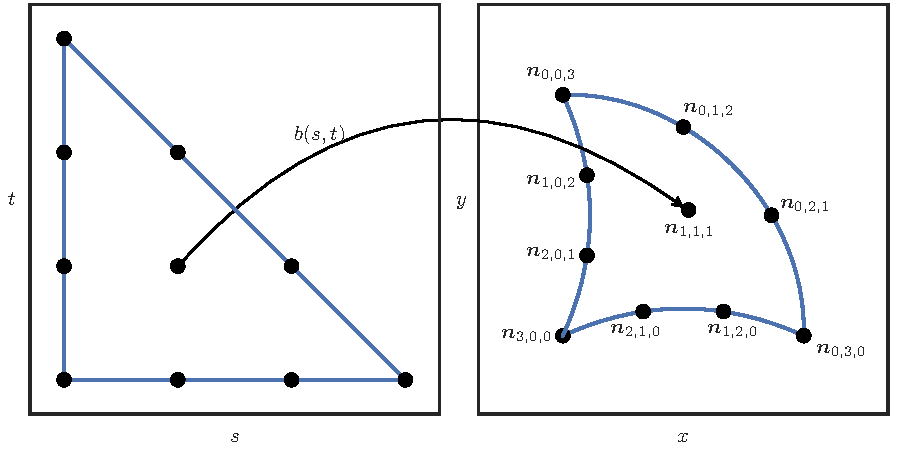
\includegraphics[width=0.9375\textwidth]{../images/curved-mesh/main_figure01.pdf}
  \centering
  \caption{Cubic B\'{e}zier triangle}
  \label{fig:cubic-bezier-example}
\end{figure}

\noindent Rather than defining a B\'{e}zier triangle by the control net, it can
also be uniquely determined by the image of a standard lattice of
points in \(\utri\): \(b\left(j/n, k/n\right) = \mathbf{n}_{i, j, k}\);
we'll refer to these as \textbf{standard nodes}.
Figure~\ref{fig:cubic-bezier-example} shows these standard nodes for
a cubic triangle. To see the correspondence,
when \(p = 1\) the standard nodes \textbf{are} the control net
\begin{equation}
b(s, t) = \lambda_1 \mathbf{n}_{1, 0, 0} +
\lambda_2 \mathbf{n}_{0, 1, 0} + \lambda_3 \mathbf{n}_{0, 0, 1}
\end{equation}
and when \(p = 2\)
\begin{multline}
b(s, t) = \lambda_1\left(2 \lambda_1 - 1\right) \mathbf{n}_{2, 0, 0} +
\lambda_2\left(2 \lambda_2 - 1\right) \mathbf{n}_{0, 2, 0} +
\lambda_3\left(2 \lambda_3 - 1\right) \mathbf{n}_{0, 0, 2} + \\
4 \lambda_1 \lambda_2 \mathbf{n}_{1, 1, 0} +
4 \lambda_2 \lambda_3 \mathbf{n}_{0, 1, 1} +
4 \lambda_3 \lambda_1 \mathbf{n}_{1, 0, 1}.
\end{multline}
However, it's worth noting that the transformation between
the control net and the standard nodes has condition
number that grows exponentially with \(n\) (see~\cite{Farouki1991}).
This may make working with
higher degree triangles prohibitively unstable.

\section{Curved Elements}

We define a curved mesh element \(\mathcal{T}\) of degree \(p\)
to be a B\'{e}zier triangle in \(\mathbf{R}^2\) of the same degree.
We refer to the component functions of \(b(s, t)\) (the map that
defined \(\mathcal{T}\)) as \(x(s, t)\) and \(y(s, t)\).

\subsection{Shape Functions}

When defining shape functions (i.e. a basis with geometric meaning) on a
curved element there are (at least) two choices. When the degree of the
shape functions is the same as the degree of the B\'{e}zier triangle,
we say the element \(\mathcal{T}\) is \textbf{isoparametric}.
For the multi-index
\(\mathbf{i} = (i, j , k)\), we define \(\mathbf{u}_{\mathbf{i}} =
\left(j/n, k/n\right)\) and the corresponding standard node
\(\mathbf{n}_{\mathbf{i}} = b\left(\mathbf{u}_{\mathbf{i}}\right)\).
Given these points, two choices for shape functions present
themselves:
\begin{itemize}
  \item \textbf{Pre-Image Basis}:
    \(\varphi_{\mathbf{j}}\left(\mathbf{n}_{\mathbf{i}}\right) =
      \widehat{\varphi}_{\mathbf{j}}\left(\mathbf{u}_{\mathbf{i}}\right) =
      \widehat{\varphi}_{\mathbf{j}}\left(b^{-1}\left(
      \mathbf{n}_{\mathbf{i}}\right)\right)\)
    where \(\widehat{\varphi}_{\mathbf{j}}\) is a canonical basis function
    on \(\utri\), i.e.
    \(\widehat{\varphi}_{\mathbf{j}}\) a degree \(p\) bivariate polynomial and
    \(\widehat{\varphi}_{\mathbf{j}}\left(\mathbf{u}_{\mathbf{i}}\right) =
    \delta_{\mathbf{i} \mathbf{j}}\)
  \item \textbf{Global Coordinates Basis}:
    \(\varphi_{\mathbf{j}}\left(\mathbf{n}_{\mathbf{i}}\right) =
    \delta_{\mathbf{i} \mathbf{j}}\), i.e. a canonical basis function
    on the standard nodes \(\left\{\mathbf{n}_{\mathbf{i}}\right\}\).
\end{itemize}

\noindent For example, consider a quadratic B\'{e}zier triangle:
\begin{gather}
b(s, t) = \left[ \begin{array}{c c}
    4 (s t + s + t) & 4 (s t + t + 1)
  \end{array}\right]^T \\
\Longrightarrow
\left[ \begin{array}{c c c c c c}
    \mathbf{n}_{2, 0, 0} &
    \mathbf{n}_{1, 1, 0} &
    \mathbf{n}_{0, 2, 0} &
    \mathbf{n}_{1, 0, 1} &
    \mathbf{n}_{0, 1, 1} &
    \mathbf{n}_{0, 0, 2}
  \end{array}\right] = \left[ \begin{array}{c c c c c c}
    0 & 2 & 4 & 2 & 5 & 4 \\
    4 & 4 & 4 & 6 & 7 & 8
  \end{array}\right].
\end{gather}
In the \textbf{Global Coordinates Basis}, we have
\begin{equation}
\varphi^{G}_{0, 1, 1}(x, y) = \frac{(y - 4) (x - y + 4)}{6}.
\end{equation}
For the \textbf{Pre-Image Basis}, we need the inverse
and the canonical basis
\begin{equation}
b^{-1}(x, y) = \left[ \begin{array}{c c}
    \frac{x - y + 4}{4} & \frac{y - 4}{x - y + 8}
  \end{array}\right] \quad \text{and} \quad
\widehat{\varphi}_{0, 1, 1}(s, t) = 4 s t
\end{equation}
and together they give
\begin{equation}
\varphi^{P}_{0, 1, 1}(x, y) = \frac{(y - 4) (x - y + 4)}{x - y + 8}.
\end{equation}
In general \(\varphi_{\mathbf{j}}^P\) may not even be a rational bivariate
function; due to composition with \(b^{-1}\) we can only guarantee that
it is algebraic (i.e. it can be defined as the zero set of polynomials).

\subsection{Curved Polygons}

\begin{figure}
  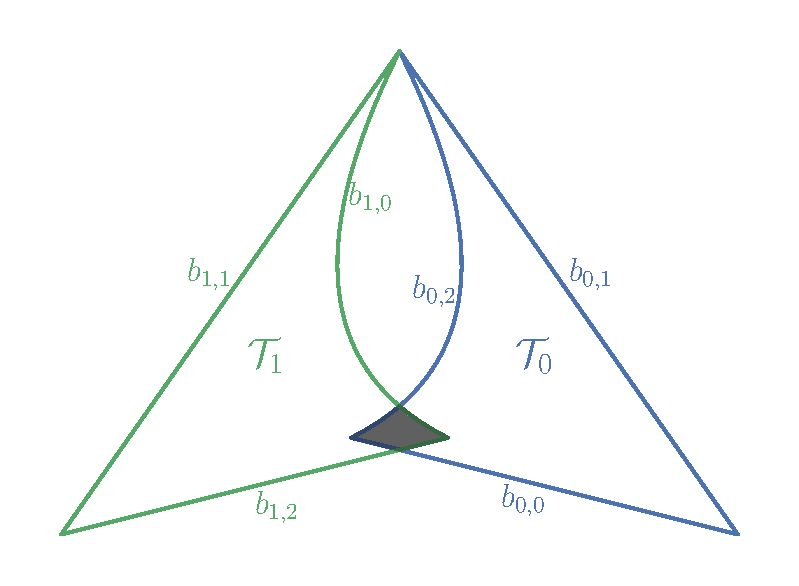
\includegraphics[width=0.625\textwidth]{../images/curved-mesh/main_figure26.pdf}
  \centering
  \caption{Intersection of B\'{e}zier triangles}
  \label{fig:bezier-triangle-intersect}
\end{figure}

When intersecting two curved elements, the resulting surface will
be defined by the boundary, alternating between edges of each
element.
For example, in Figure~\ref{fig:bezier-triangle-intersect}, a
``curved quadrilateral'' is formed when two B\'{e}zier triangles
\(\mathcal{T}_0\) and \(\mathcal{T}_1\) are intersected.

A \textbf{curved polygon} is defined by a collection of B\'{e}zier curves
in \(\mathbf{R}^2\) that determine the boundary. In order to be
a valid polygon, none of the boundary curves may cross and the
ends of consecutive edge curves must meet. For our example in
Figure~\ref{fig:bezier-triangle-intersect}, the triangles
have boundaries formed by three B\'{e}zier curves:
\(\partial \mathcal{T}_0 = b_{0, 0} \cup b_{0, 1} \cup b_{0, 2}\) and
\(\partial \mathcal{T}_1 = b_{1, 0} \cup b_{1, 1} \cup b_{1, 2}\).
The intersection \(\mathcal{I}\) is defined by its boundary\footnote{Each
specialization of a B\'{e}zier curve \(b\left(\left[a_1, a_2\right]\right)\)
is itself a B\'{e}zier curve.}:
\begin{equation}
\partial \mathcal{I} = b_{0, 0}\left(\left[0, 1/8\right]\right) \cup
  b_{1, 2}\left(\left[7/8, 1\right]\right) \cup
  b_{1, 0}\left(\left[0, 1/7\right]\right) \cup
  b_{0, 2}\left(\left[6/7, 1\right]\right).
\end{equation}

Though an intersection can be described in terms of the B\'{e}zier triangles,
the structure of the control net will be lost. The region will not in general
be able to be described by a mapping from a simple space like
\(\utri\).

\section{Floating Point and Forward Error Analysis}

We assume all floating point operations obey
\begin{equation}
  a \star b = \fl{a \circ b} = (a \circ b)(1 + \delta_1) =
  (a \circ b) / (1 + \delta_2)
\end{equation}
where \(\star \in \left\{\oplus, \ominus, \otimes, \oslash\right\}\), \(\circ
\in \left\{+, -, \times, \div\right\}\) and \(\left|\delta_1\right|,
\left|\delta_2\right| \leq \mach\). The symbol \(\mach\) is the unit round-off
and \(\star\) is a floating point operation, e.g.
\(a \oplus b = \fl{a + b}\). (For IEEE-754 floating point double precision,
\(\mach = 2^{-53}\).) We denote the computed result of
\(\alpha \in \mathbf{R}\) in floating point arithmetic by
\(\widehat{\alpha}\) or \(\fl{\alpha}\) and use \(\mathbf{F}\) as the set of
all floating point numbers (see \cite{Higham2002} for more details).
Following \cite{Higham2002}, we will use the following classic properties in
error analysis.

\begin{enumerate}
  \item If \(\delta_i \leq \mach\), \(\rho_i = \pm 1\), then
      \(\prod_{i = 1}^n (1 + \delta_i)^{\rho_i} = 1 + \theta_n\),
  \item \(\left|\theta_n\right| \leq \gamma_n \coloneqq
      n \mach / (1 - n \mach)\),
  \item \((1 + \theta_k)(1 + \theta_j) = 1 + \theta_{k + j}\),
  \item \(\gamma_k + \gamma_j + \gamma_k \gamma_j \leq \gamma_{k + j}
    \Longleftrightarrow (1 + \gamma_k)(1 + \gamma_j) \leq 1 + \gamma_{k + j}\),
  \item \((1 + \mach)^j \leq 1 / (1 - j \mach) \Longleftrightarrow
  (1 + \mach)^j - 1 \leq \gamma_j\).
\end{enumerate}

\section{Error-Free Transformation}

An error-free transformation is a computational method where both
the computed result and the round-off error are returned. It
is considered ``free'' of error if the round-off can be represented
exactly as an element or elements of \(\mathbf{F}\).
The error-free transformations used in this paper are
the \texttt{TwoSum} algorithm by Knuth (\cite{Knuth1997}) and
\texttt{TwoProd} algorithm by Dekker (\cite{Dekker1971}, Section 5),
respectively.

\begin{theorem}[\cite{Ogita2005}, Theorem 3.4]\label{thm:eft}
For \(a, b \in \mathbf{F}\) and \(P, \pi, S, \sigma \in \mathbf{F}\),
\texttt{TwoSum} and \texttt{TwoProd} satisfy
\begin{alignat}{4}
\left[S, \sigma\right] &= \mathtt{TwoSum}(a, b), & \, S &= \fl{a + b},
  S + \sigma &= a + b, \sigma &\leq \mach \left|S\right|,
  & \, \sigma &\leq \mach \left|a + b\right| \\
\left[P, \pi\right] &= \mathtt{TwoProd}(a, b),
  & \, P &= \fl{a \times b}, P + \pi &= a \times b,
  \pi &\leq \mach \left|P\right|,
  & \, \pi &\leq \mach \left|a \times b\right|.
\end{alignat}
The letters \(\sigma\) and \(\pi\) are used to indicate that the
errors came from sum and product, respectively. See
Appendix~\ref{chap:appendix-algo} for implementation details.
\end{theorem}

\section{de Casteljau Algorithm}

Next, we recall\footnote{We have used slightly non-standard notation for the
terms produced by the de Casteljau algorithm: we start the superscript at
\(n\) and count down to \(0\) as is typically done when describing Horner's
algorithm. For example, we use \(b_j^{(n - 2)}\) instead of
\(b_j^{(2)}\).} the de Casteljau algorithm:

\begin{breakablealgorithm}
  \caption{\textit{de Casteljau algorithm for polynomial evaluation.}}
  \label{alg:de-casteljau}

  \begin{algorithmic}
    \Function{\(\mathtt{result} = \mathtt{DeCasteljau}\)}{$b, s$}
      \State \(n = \texttt{length}(b) - 1\)
      \State \(\widehat{r} = 1 \ominus s\)
      \\
      \For{\(j = 0, \ldots, n\)}
        \State \(\widehat{b}_j^{(n)} = b_j\)
      \EndFor
      \\
      \For{\(k = n - 1, \ldots, 0\)}
        \For{\(j = 0, \ldots, k\)}
          \State \(\widehat{b}_j^{(k)} = \left(
              \widehat{r} \otimes \widehat{b}_j^{(k + 1)}\right) \oplus
              \left(s \otimes \widehat{b}_{j + 1}^{(k + 1)}\right)\)
        \EndFor
      \EndFor
      \\
      \State \(\mathtt{result} = \widehat{b}_0^{(0)}\)
    \EndFunction
  \end{algorithmic}
\end{breakablealgorithm}

\begin{theorem}[\cite{Mainar1999}, Corollary 3.2]
If \(p(s) = \sum_{j = 0}^n b_j B_{j, n}(s)\) and \(\mathtt{DeCasteljau}(p, s)\)
is the value computed by the de Casteljau algorithm then\footnote{In the
original paper the factor on \(\widetilde{p}(s)\) is \(\gamma_{2n}\),
but the authors did not consider round-off when computing
\(1 \ominus s\).}
\begin{equation}
\left|p(s) - \mathtt{DeCasteljau}(p, s)\right| \leq \gamma_{3n}
\sum_{j = 0}^n \left|b_j\right| B_{j, n}(s).
\end{equation}
\end{theorem}

The relative condition number of the evaluation of \(p(s) = \sum_{j = 0}^n
b_j B_{j, n}(s)\) in Bernstein form used in this paper is (see
\cite{Mainar1999}, \cite{Farouki1987}):
\begin{equation}
\cond{p, s} = \frac{\widetilde{p}(s)}{\left|p(s)\right|},
\end{equation}
where
\(\widetilde{p}(s) \coloneqq \sum_{j = 0}^n \left|b_j\right| B_{j, n}(s)\).

To be able to express the algorithm in matrix form, we define
the vectors
\begin{equation}
b^{(k)} = \left[\begin{array}{c c c} b_0^{(k)} & \cdots &
b_k^{(k)}\end{array}\right]^T, \quad
\widehat{b}^{(k)} = \left[\begin{array}{c c c} \widehat{b}_0^{(k)} & \cdots &
    \widehat{b}_k^{(k)}\end{array}\right]^T
\end{equation}
and the reduction matrices:
\begin{equation}
U_k = U_k(s) = \left[\begin{array}{c c c c c c}
    1 - s  & s      & 0      & \cdots & \cdots & 0      \\
    0      & 1 - s  & s      & \ddots &        & \vdots \\
    \vdots & \ddots & \ddots & \ddots & \ddots & \vdots \\
    \vdots &        & \ddots & \ddots & \ddots & 0 \\
    0      & \cdots & \cdots & 0      & 1 - s  & s
\end{array}\right] \in \mathbf{R}^{k \times (k + 1)}.
\end{equation}
With this, we can express (\cite{Mainar1999}) the de Casteljau algorithm as
\begin{equation}\label{matrix-de-casteljau}
b^{(k)} = U_{k + 1} b^{(k + 1)}
\Longrightarrow b^{(0)} = U_1 \cdots U_n b^{(n)}.
\end{equation}

In general, for a sequence \(v_0, \ldots, v_n\) we'll refer to \(v\)
as the vector containing all of the values:
\(v = \left[\begin{array}{c c c} v_0 & \cdots &
    v_n\end{array}\right]^T.\)
